\newpage
%=====================================================================================
%
%                    POSLEDNÍ ITERACE 
%
%
%======================================================================================
% MODELY 1. ITERACE %
% === FRONT PAGE ===
\thispagestyle{plain}
	\newgeometry{left=2cm,right=2cm,top=1.5cm}
	\pagenumbering{gobble}
	\begin{center}
		\Huge
		VYSOKÉ UČENÍ TECHNICKÉ V BRNĚ \\
			\vspace{\stretch{0.150}}


	
\includegraphics[width=\textwidth]{resources/fit-logo.pdf}
			\vspace{\stretch{0.300}}



		\Large{Projekt do předmětu AIS \\ ~ \\}
		
		\LARGE
		\textsc{Výsledné modely}
			\vspace{\stretch{0.618}}

	\end{center}

	\noindent \textbox{5. prosince, 2017} \textbox{\hfill \textbf{Autoři:}  Daniel Dušek ~~(xdusek21) ~~~}
	\noindent \textbox{\hfill} \textbox{\hfill Filip Kalous ~~~(xkalou03) ~~~}
	\noindent \textbox{\hfill} \textbox{\hfill Anna Popková (xpopko00)~~~}

	\clearpage
	\restoregeometry

\newpage

\normalsize



%%%%%%%%%%%%%%%%%%%%%%%
% Potvrzení rezervace %  
%%%%%%%%%%%%%%%%%%%%%%%
\section*{Specifikace případů užití}
\textbf{Případ užití \uv{Potvrdit rezervaci}}
\begin{table}[ht!]
{\renewcommand{\arraystretch}{1.3}
\begin{tabular}{| r | p{12cm} |}
	\hline
	ID: & 4 \\
    \hline
    Název: & \textbf{Potvrdit rezervaci} \\
    \hline
    Vytvořeno: & Filip Kalous, Daniel Dušek, Anna Popková \\
    \hline
    Popis: & Kancelář potvrdí rezervaci vytvořenou zákazníkem \\
    \hline
    Primární aktéři: & Kancelář, Systém \\
    \hline
    Sekundární aktéři: & Zákazník \\
    \hline
    Předpoklady: & Zákazník někdy v minulosti vytvořil žádost o rezervaci, která nebyla zamítnuta systémem, ani zpracována pracovníkem Kancelář. \\
    \hline
    Následné podmínky: & 
    \begin{minipage}[t]{0.75\textwidth}
    	\begin{enumerate}[nosep,after=\strut]
    		\item V systému je potvrzena rezervace zákazníka.
            \item Zákazníkovi je na email zaslán rezervační klíč.
    	\end{enumerate}
  	\end{minipage} \\
	\hline
    Akce pro spuštění: & Kancelář má zobrazený seznam rezervací, které čekají na potvrzení. \\
    \hline
    Hlavní tok: & 
    \begin{minipage}[t]{0.75\textwidth}
    	\begin{enumerate}[nosep,after=\strut]
            %\item Aktér Kancelář klikne na odkaz \uv{Potvrzovat rezervace}.
            %\item Systém zobrazí uživateli seznam vytvořených rezervací, které čekají na potvrzení.
            \item Aktér Kancelář vybere ze seznamu čekajících rezervací tu, kterou chce potvrdit a klikne u ní na tlačítko \uv{Potvrdit rezervaci}.
            \item Systém zkontroluje zda jsou splněny všechny podmínky, za kterých může být rezervace potvrzena a podmínky jsou úspěšně splněny.
            \item Systém vygeneruje unikátní identifikátor rezervace a \uv{Storno} odkaz, který zašle na email Zákazníka vytvářejícího rezervaci.
            \item Systém zobrazí informaci o potvrzení rezervace.
    	\end{enumerate}
  	\end{minipage} \\
    \hline 
    Alternativní toky: & Rezervované místo není k dispozici  \\
    \hline
    Výjimky: & 
    \begin{minipage}[t]{0.75\textwidth}
    	\begin{enumerate}[nosep,after=\strut] 
            \item Selhání systému
            \item Selhání operace
            \item Selhání služby odesílající email
    	\end{enumerate}
  	\end{minipage} \\
    \hline
    Frekvence: & Často \\
    \hline
    Speciální požadavky: & 
    \begin{minipage}[t]{0.75\textwidth}
    	\begin{enumerate}[nosep,after=\strut]
    		\item Žádné
    	\end{enumerate}
  	\end{minipage} \\
    \hline
\end{tabular}}
\caption{Specifikace případu užití \uv{Potvrdit rezervaci}}
\label{table:1}
\end{table}

%%%%%%%%%%%%%%%%%%%%%%%%%%%%%%%%%%%%%%%%%%%%%%%%%%%%%%%%%%
% Alternativní tok -  Rezervované místo není k dispozici %  
%%%%%%%%%%%%%%%%%%%%%%%%%%%%%%%%%%%%%%%%%%%%%%%%%%%%%%%%%%
\newpage
\textbf{Alternativní tok případu užití: \uv{Rezervované místo není k dispozici}}
\begin{table}[ht!]
{\renewcommand{\arraystretch}{1.3}
\begin{tabular}{| r | p{12cm} |}
	\hline
	ID: & 4.1 \\
    \hline
    Název: & \textbf{Potvrdit rezervaci: Rezervované místo není k dispozici.} \\
    \hline
    Vytvořeno: & Filip Kalous, Daniel Dušek, Anna Popková \\
    \hline
    Popis: & Rezervace není potvrzena z důvodu nedostupného místa. \\
    \hline
    Primární aktéři: & Kancelář, Systém \\
    \hline
    Sekundární aktéři: &  \\
    \hline
    Předpoklady: & V době potvrzování rezervace systém zjistí, že vybraná místa nejsou již k dispozici.  \\
    \hline
    Následné podmínky: & 
	\begin{minipage}[t]{0.75\textwidth}
 		\begin{enumerate}[nosep,after=\strut]
 			\item Rezervace je automaticky zamítnuta.
 			\item Zákazník je informován o tom, že jeho rezervace byla zamítnuta.
            \item Pracovník Kanceláře je informován o skutečnosti, že rezervace byla zamítnuta, včetně informace o důvodu automatického zamítnutí.
 		\end{enumerate}
    \end{minipage} \\
	\hline
    Akce pro spuštění: & Kliknutí na tlačítko Potvrdit rezervaci u rezervace, která obsahuje nedostupné místo. \\
    \hline
    Tok: & 
    \begin{minipage}[t]{0.75\textwidth}
    	\begin{enumerate}[nosep,after=\strut]
            \item Aktér Kancelář klikne na odkaz \uv{Potvrzovat rezervace}.
            \item Systém zobrazí uživateli seznam vytvořených rezervací, které čekají na potvrzení.
            \item Aktér Kancelář vybere ze seznamu čekajících rezervací tu, kterou chce potvrdit a klikne na tlačítko \uv{Potvrdit rezervaci}.
            \item Systém zkontroluje zda jsou splněny všechny podmínky, za kterých může být rezervace potvrzena a podmínky nejsou úspěšně splněny. Některé z rezervovaných míst je již obsazeno jinou rezervací.
            \item Systém vygeneruje email informující uživatele o zamítnutí jeho rezervace.
            \item Systém zobrazí informaci o automatickém zamítnutí rezervace, včetně důvodů.
    	\end{enumerate}
    \end{minipage} \\
    \hline
    Frekvence: & Málo často \\
    \hline
    Speciální požadavky: & 
    \begin{minipage}[t]{0.75\textwidth}
    	\begin{enumerate}[nosep,after=\strut]
    		\item Aktér Kancelář pracoval s více instancemi aplikace (například otevřenými taby prohlížeče) a některou ze vzájemně konfliktních rezervací potvrdil na první instanci a druhou konfliktní se pokusil potvrdit v druhé instanci.
    	\end{enumerate}
  	\end{minipage} \\
    \hline
\end{tabular}}
\caption{Potvrdit rezervaci: Rezervované místo není k dispozici}
\label{table:2}
\end{table}

%%%%%%%%%%%%%%%%%%%%%%%
% Výjimka 1&2 - Selhání systému, selhání odesílání mailu %  
%%%%%%%%%%%%%%%%%%%%%%%
\textbf{Výjimka \textit{4.E.1 Selhání systému} je popsána již v 1.E.3 z modelů případů použití v první iteraci.} \\
\newpage
\textbf{Výjimka \textit{Selhání služby odesílající email}}:
\begin{center}
\begin{table}[ht!]
{\renewcommand{\arraystretch}{1.3}
\begin{tabular}{| r | p{12cm} |}
	\hline
	ID: & 4.E.2\\
    \hline
    Název: & \textbf{Potvrdit rezervaci: Selhání služby odesílající email} \\
    \hline
    Vytvořeno: & Filip Kalous, Daniel Dušek, Anna Popková \\
    \hline
    Popis: & Systém potvrdí/zamítne rezervaci, ale není schopen odeslat informační email. \\
    \hline
    Primární aktéři: & Systém \\
    \hline
    Sekundární aktéři: &  Kancelář \\
    \hline
    Předpoklady: & 
    \begin{minipage}[t]{0.75\textwidth}
    	\begin{enumerate}[nosep,after=\strut]
    		\item Modul systému zodpovědný za odesílání emailu nezvládl odeslat email.
            \item Systém nespadl a potvrzení/zamítnutí rezervace provedl.
    	\end{enumerate}
  	\end{minipage} \\
    \hline
    Následné podmínky: & 
    \begin{minipage}[t]{0.75\textwidth}
    	\begin{enumerate}[nosep,after=\strut]
    		\item Systém neodeslal informační email uživateli.
            \item Systém informoval aktéra Kancelář o neúspěšném odeslání emailu.
            \item Systém poskytl informace aktérovi Kancelář pro maniální odeslání mailu.
    	\end{enumerate}
  	\end{minipage} \\
	\hline
    Akce pro spuštění: & Selhání systému v libovolném místě toku případu \uv{Vytvořit rezervaci}. \\
    \hline
    Tok: & 
    \begin{minipage}[t]{0.75\textwidth}
    	\begin{enumerate}[nosep,after=\strut]
            \item Systém v průběhu vykonávání potvrzení/zamítnutí rezervace generuje obsah emailu pro Zákazníka vytvářejícího rezervaci.
            \item Systém kontaktuje svůj modul pro odeslání emailu a vyžádá si odeslání mailu Zákazníkovi.
            \item Odeslání emailu selže.
            \item Systém zobrazí informační hlášku aktérovi Kancelář informující ho o neúspěchu odesílání emailu. V informační hlášce je obsažen text emailu a adresa na kterou měl být původně zaslán a doporučení provedení tohoto kroku manuálně, mimo systém.
    	\end{enumerate}
  	\end{minipage} \\
    \hline
    Frekvence: & Velice zřídka \\
    \hline

\end{tabular}}
\caption{Vytvořit rezervaci: Selhání služby odesílající email}
\label{table:4}
\end{table}
\end{center}

\newpage
%%%%%%%%%%%%%%%%%%%%%%%%%%
%     USE CASE 5         %
%%%%%%%%%%%%%%%%%%%%%%%%%%
% ZADAT OBJEDNAVKU %
\textbf{Případ užití \uv{Zadat objednávku}}
\begin{table}[ht!]
{\renewcommand{\arraystretch}{1.3}
\begin{tabular}{| r | p{12cm} |}
	\hline
	ID: & 5 \\
    \hline
    Název: & \textbf{Zadat objednávku} \\
    \hline
    Vytvořeno: & Filip Kalous, Daniel Dušek, Anna Popková \\
    \hline
    Popis: & Obslužný personál zadá do systému objednávku a přiřadí ji ke stolu. \\
    \hline
    Primární aktéři: & Oblužný personál\\
    \hline
    Sekundární aktéři: & Systém  \\
    \hline
    Předpoklady: & Zákazník u stolu provedl mimo systém objednávku (například ústně) a obslužný personál zadává do systému informaci o jeho objednávce.  \\
    \hline
    Následné podmínky: & 
    \begin{minipage}[t]{0.75\textwidth}
    	\begin{enumerate}[nosep,after=\strut]
    		\item V systému je vytvořena objednávka.
            \item Vytvořená objednávka je svázána se stolem ke kterému má být doručována.
    	\end{enumerate}
  	\end{minipage} \\
	\hline
    Akce pro spuštění: & Obslužný personál zapne režim \uv{Zadávání objednávky} \\
    \hline
    Hlavní tok: & 
    \begin{minipage}[t]{0.75\textwidth}
    	\begin{enumerate}[nosep,after=\strut]
            \item Aktér Obslužný personál klikne na tlačítko \uv{Zadat objednávku}.
            \item Systém zobrazí uživatelské rozhraní pro zadávání objednávky obsahující (mimo jiné) možnost specifikace stolu, ke kterému se objednávka vztahuje.
            \item Aktér Obslužný personál zadá obsah objednávky a klikne na tlačítko \uv{Zadat}
            \item Systém zkontroluje že Obslužný personál vybral stůl ke kterému se objednávka vztahuje. Tato kontrola proběhne úspěšně.
            \item Systém vytvoří v systému objednávku se všemi zadanými informacemi od obsluhy.
    	\end{enumerate}
  	\end{minipage} \\
    \hline 
    Alternativní toky: & Oblužný personál nezadá objednávající stůl  \\
    \hline
    Výjimky: & 
    \begin{minipage}[t]{0.75\textwidth}
    	\begin{enumerate}[nosep,after=\strut] 
            \item Selhání systému
            \item Selhání operace
    	\end{enumerate}
  	\end{minipage} \\
    \hline
    Frekvence: & Často \\
    \hline
    Speciální požadavky: & 
    \begin{minipage}[t]{0.75\textwidth}
    	\begin{enumerate}[nosep,after=\strut]
    		\item Žádné
    	\end{enumerate}
  	\end{minipage} \\
    \hline

\end{tabular}}
\caption{Specifikace případu užití \uv{Zadat objednávku}}
\label{table:1}
\end{table}

\newpage
% ALTERNATIVNI TOK - NEZADANY STUl % 
\begin{table}[ht!]
{\renewcommand{\arraystretch}{1.3}
\begin{tabular}{| r | p{12cm} |}
	\hline
	ID: & 5.1 \\
    \hline
    Název: & \textbf{Zadat objednávku: Oblužný personál nezadá objednávající stůl} \\
    \hline
    Vytvořeno: & Filip Kalous, Daniel Dušek, Anna Popková \\
    \hline
    Popis: & Oblužný personál zadává objednávku bez vyplněného stolu. \\
    \hline
    Primární aktéři: & Obslužný personál, Systém \\
    \hline
    Sekundární aktéři: &  \\
    \hline
    Předpoklady: & Oblužný personál přijal objednávku a zadává ji do systému.  \\
    \hline
    Následné podmínky: & 
	\begin{minipage}[t]{0.75\textwidth}
 		\begin{enumerate}[nosep,after=\strut]
 			\item Systém nevytvoří objednávku u které by nebyl vybraný stůl ke kterému se vztahuje.
            \item Systém navede Obslužný personál aby dokončil zadávání objednávky úspěšně.
 		\end{enumerate}
    \end{minipage} \\
	\hline
    Akce pro spuštění: & Obslužný personál zapne režim \uv{Zadávání objednávky}, zadá objednávku a nevyplní stůl, ke kterému se vztahuje a potvrdí zadávání. \\
    \hline
    Tok: & 
    \begin{minipage}[t]{0.75\textwidth}
    	\begin{enumerate}[nosep,after=\strut]
            \item Aktér Obslužný personál klikne na tlačítko \uv{Zadat objednávku}.
            \item Systém zobrazí uživatelské rozhraní pro zadávání objednávky obsahující (mimo jiné) možnost specifikace stolu, ke kterému se objednávka vztahuje.
            \item Aktér Obslužný personál zadá obsah objednávky bez vyplněného objednávajícího stolu a klikne na tlačítko \uv{Zadat}
            \item Systém zkontroluje že Obslužný personál vybral stůl ke kterému se objednávka vztahuje. Tato kontrola proběhne neúspěšně, protože stůl nebyl vyplněn.
            \item Systém zobrazí chybovou hlášku o chybějícím stolu, ke kterému se objednávka vztahuje a informací pro Obslužný personál, jak tuto informaci doplnil.
            \item Obslužný personál doplní informaci a znovu klikne na tlačítko \uv{Zadat}
            \item Tok dále pokračuje od bodu 4 standardního případu použití.
    	\end{enumerate}
    \end{minipage} \\
    \hline
    Frekvence: & Středně \\
    \hline
    Speciální požadavky: & \\  
        \hline

\end{tabular}}
\caption{Zadat objednávku: Rezervované místo není k dispozici}
\label{table:2}
\end{table}

%%%%%%%%%%%%%%%%%%%%%%%%%%%%%%%
%        USE CASE 6           %
%%%%%%%%%%%%%%%%%%%%%%%%%%%%%%%
\newpage
% Stornovat rezervaci %
\textbf{Případ užití: \uv{Stornovat rezervaci}}
\begin{table}[ht!]
{\renewcommand{\arraystretch}{1.3}
\begin{tabular}{| r | p{12cm} |}
	\hline
	ID: & 6 \\
    \hline
    Název: & \textbf{Stornovat rezervaci} \\
    \hline
    Vytvořeno: & Filip Kalous, Daniel Dušek, Anna Popková \\
    \hline
    Popis: & Zákazník stornuje svou rezervaci \\
    \hline
    Primární aktéři: & Zákazník \\
    \hline
    Sekundární aktéři: & Systém \\
    \hline
    Předpoklady: & Zákazník si vytvořil rezervaci, která je čekající na potvrzení, nebo je již potvrzená. \\
    \hline
    Následné podmínky: & 
    \begin{minipage}[t]{0.75\textwidth}
    	\begin{enumerate}[nosep,after=\strut]
    		\item Rezervace, kterou chtěl Zákazník stornovat je stornována.
            \item Stoly nebo salón, které byly předmětem rezervace jsou opět uvolněny k možné rezervaci.
    	\end{enumerate}
  	\end{minipage} \\
	\hline
    Akce pro spuštění: & Zákazník klikne na odkaz \uv{Stornovat rezervaci} \\
    \hline
    Hlavní tok: & 
    \begin{minipage}[t]{0.75\textwidth}
    	\begin{enumerate}[nosep,after=\strut]
            \item Zákazník klikne na odkaz \uv{Stornovat rezervaci} a je přesměrován na stránku s formulářem pro stornování rezervace.
            \item Zákazník vyplní ve formuláři rezervační klíč a klepne na tlačítko \uv{Stornovat rezervaci}
            \item Zákazník potvrdí, že chce rezervaci opravdu stornovat.
            \item Systém zkontroluje, zda rezervace s poskytnutým klíčem existuje a zda ještě nenastal její čas. Kontrola proběhne úspěšně.
            \item Systém uvolní registrované stoly, popřípadě salónek v době stornované rezervace.
            \item Systém odstraní rezervaci ze systému. 
    	\end{enumerate}
  	\end{minipage} \\
    \hline
    Alternativní toky: & 
    \begin{minipage}[t]{0.75\textwidth}
    	\begin{enumerate}[nosep,after=\strut]
            \item Zákazník vyplní špatný rezervační klíč.
            \item Zákazník vyplní rezervační klíče rezervace, která již započala.
    	\end{enumerate}
  	\end{minipage} \\
    \hline
    Výjimky: & 
    \begin{minipage}[t]{0.75\textwidth}
    	\begin{enumerate}[nosep,after=\strut]
    		\item Selhání systému
    		\item Selhání operace
    	\end{enumerate}
  	\end{minipage} \\
    \hline
    Frekvence: & Středně často \\
    \hline
    Speciální požadavky: & 
    \begin{minipage}[t]{0.75\textwidth}
    	\begin{enumerate}[nosep,after=\strut]
    		\item Žádné
    	\end{enumerate}
  	\end{minipage} \\
    \hline

\end{tabular}}
\caption{Specifikace případu užití \uv{Stornovat rezervaci}}
\label{table:1}
\end{table}

\newpage
% ALTERNATIVNI TOK - Špatný rezervační klíč % 
\textbf{Alternativní tok: Špatný rezervační klíč}
\begin{table}[ht!]
{\renewcommand{\arraystretch}{1.3}
\begin{tabular}{| r | p{12cm} |}
	\hline
	ID: & 6.1 \\
    \hline
    Název: & \textbf{Stornovat rezervaci: Zákazník vyplní špatný rezervační klíč}. \\
    \hline
    Vytvořeno: & Filip Kalous, Daniel Dušek, Anna Popková \\
    \hline
    Popis: & Zákazník stornuje svou rezervaci a používá špatný rezervační klíč. \\
    \hline
    Primární aktéři: & Zákazník \\
    \hline
    Sekundární aktéři: &  Systém \\
    \hline
    Předpoklady: & Zákazník se pokouší využít funkce stornování rezervace.  \\
    \hline
    Následné podmínky: & 
	\begin{minipage}[t]{0.75\textwidth}
 		\begin{enumerate}[nosep,after=\strut]
 			\item Systém neodrezervuje žádné stoly ani salón.
            \item Systém informuje Zákazníka o důvodu neúspěchu zrušení rezervace.
 		\end{enumerate}
    \end{minipage} \\
	\hline
    Akce pro spuštění: & Zákazník odešle formulář stornující rezervaci. \\
    \hline
    Tok: & 
    \begin{minipage}[t]{0.75\textwidth}
    	\begin{enumerate}[nosep,after=\strut]
            \item Zákazník klikne na odkaz \uv{Stornovat rezervaci} a je přesměrován na stránku s formulářem pro stornování rezervace.
            \item Zákazník vyplní ve formuláři rezervační klíč a klepne na tlačítko \uv{Stornovat rezervaci}
            \item Zákazník potvrdí, že chce rezervaci opravdu stornovat.
            \item Systém zkontroluje, zda rezervace s poskytnutým klíčem existuje a zda ještě nenastal její čas. Kontrola proběhne neúspěšně, protože odpovídající rezervace se zadaným klíčem neexistuje.
            \item Systém se nepokouší uvolňovat žádné stoly ani salónek a zobrazí uživateli chybovou hlášku o špatném rezervačním klíči.
    	\end{enumerate}
    \end{minipage} \\
    \hline
    Frekvence: & Málo často \\
    \hline
    Speciální požadavky: & \\  
        \hline

\end{tabular}}
\caption{Stornovat rezervaci: Zákazník vyplní špatný rezervační klíč}
\label{table:2}
\end{table}

% ALTERNATIVNI TOK - Zákazník ruší rezervaci, která již probíhá % 
\newpage
\textbf{Alternativní tok: Zákazník ruší rezervaci, která již probíhá}
\begin{table}[ht!]
{\renewcommand{\arraystretch}{1.3}
\begin{tabular}{| r | p{12cm} |}
	\hline
	ID: & 6.2 \\
    \hline
    Název: & \textbf{Stornovat rezervaci: Zákazník vyplní rezervační klíče rezervace, která již započala.}. \\
    \hline
    Vytvořeno: & Filip Kalous, Daniel Dušek, Anna Popková \\
    \hline
    Popis: & Zákazník stornuje svou rezervaci, avšak čas aktivace rezervace již nastal. \\
    \hline
    Primární aktéři: & Zákazník \\
    \hline
    Sekundární aktéři: &  Systém, Kancelář \\
    \hline
    Předpoklady: & Zákazník se pokouší využít funkce stornování rezervace, ale jeho rezervace již začala.  \\
    \hline
    Následné podmínky: & 
	\begin{minipage}[t]{0.75\textwidth}
 		\begin{enumerate}[nosep,after=\strut]
        	\item Systém uvolní rezervované stoly, nebo salónek.
 			\item Systém zruší rezervaci.
            \item Systém informuje kancelář o tom, že probíhající rezervace byla zrušena.
 		\end{enumerate}
    \end{minipage} \\
	\hline
    Akce pro spuštění: & Zákazník odešle formulář stornující rezervaci. \\
    \hline
    Tok: & 
    \begin{minipage}[t]{0.75\textwidth}
    	\begin{enumerate}[nosep,after=\strut]
            \item Zákazník klikne na odkaz \uv{Stornovat rezervaci} a je přesměrován na stránku s formulářem pro stornování rezervace.
            \item Zákazník vyplní ve formuláři rezervační klíč a klepne na tlačítko \uv{Stornovat rezervaci}
            \item Zákazník potvrdí, že chce rezervaci opravdu stornovat.
            \item Systém zkontroluje, zda rezervace s poskytnutým klíčem existuje a zda ještě nenastal její čas. Kontrola proběhne neúspěšně, protože čas aktivace rezervace již nastal.
            \item Systém uvolní registrované stoly, popřípadě salónek v době stornované rezervace.
            \item Systém informuje Kancelář, že probíhající rezervace byla zrušena.
            \item Systém odstraní rezervaci ze systému. 
    	\end{enumerate}
    \end{minipage} \\
    \hline
    Frekvence: & Málo často \\
    \hline
    Speciální požadavky: & \\  
        \hline

\end{tabular}}
\caption{Stornovat rezervaci: Zákazník stornuje svou rezervaci, avšak čas aktivace rezervace již nastal.}
\label{table:2}
\end{table}

% JESTE VYJIMKY? %
\textbf{Výjimka 6.E.1 \textit{Selhání systému} je stejná jako výjimka 1.E.3. Výjimka 6.E.2 \textit{Selhání operace} se významově shoduje s výjimkou 1.E.4.}
\newpage


%%%%%%%%%%%%%%%%%%%%%%%%%%%%%%%%%%%%%%%%%%%%%%%%%%%%%%
%                04 SYSTEM SEQUENCE DIAGRAM          %
%%%%%%%%%%%%%%%%%%%%%%%%%%%%%%%%%%%%%%%%%%%%%%%%%%%%%%
\newpage
\begin{figure}[h!]
\begin{center}
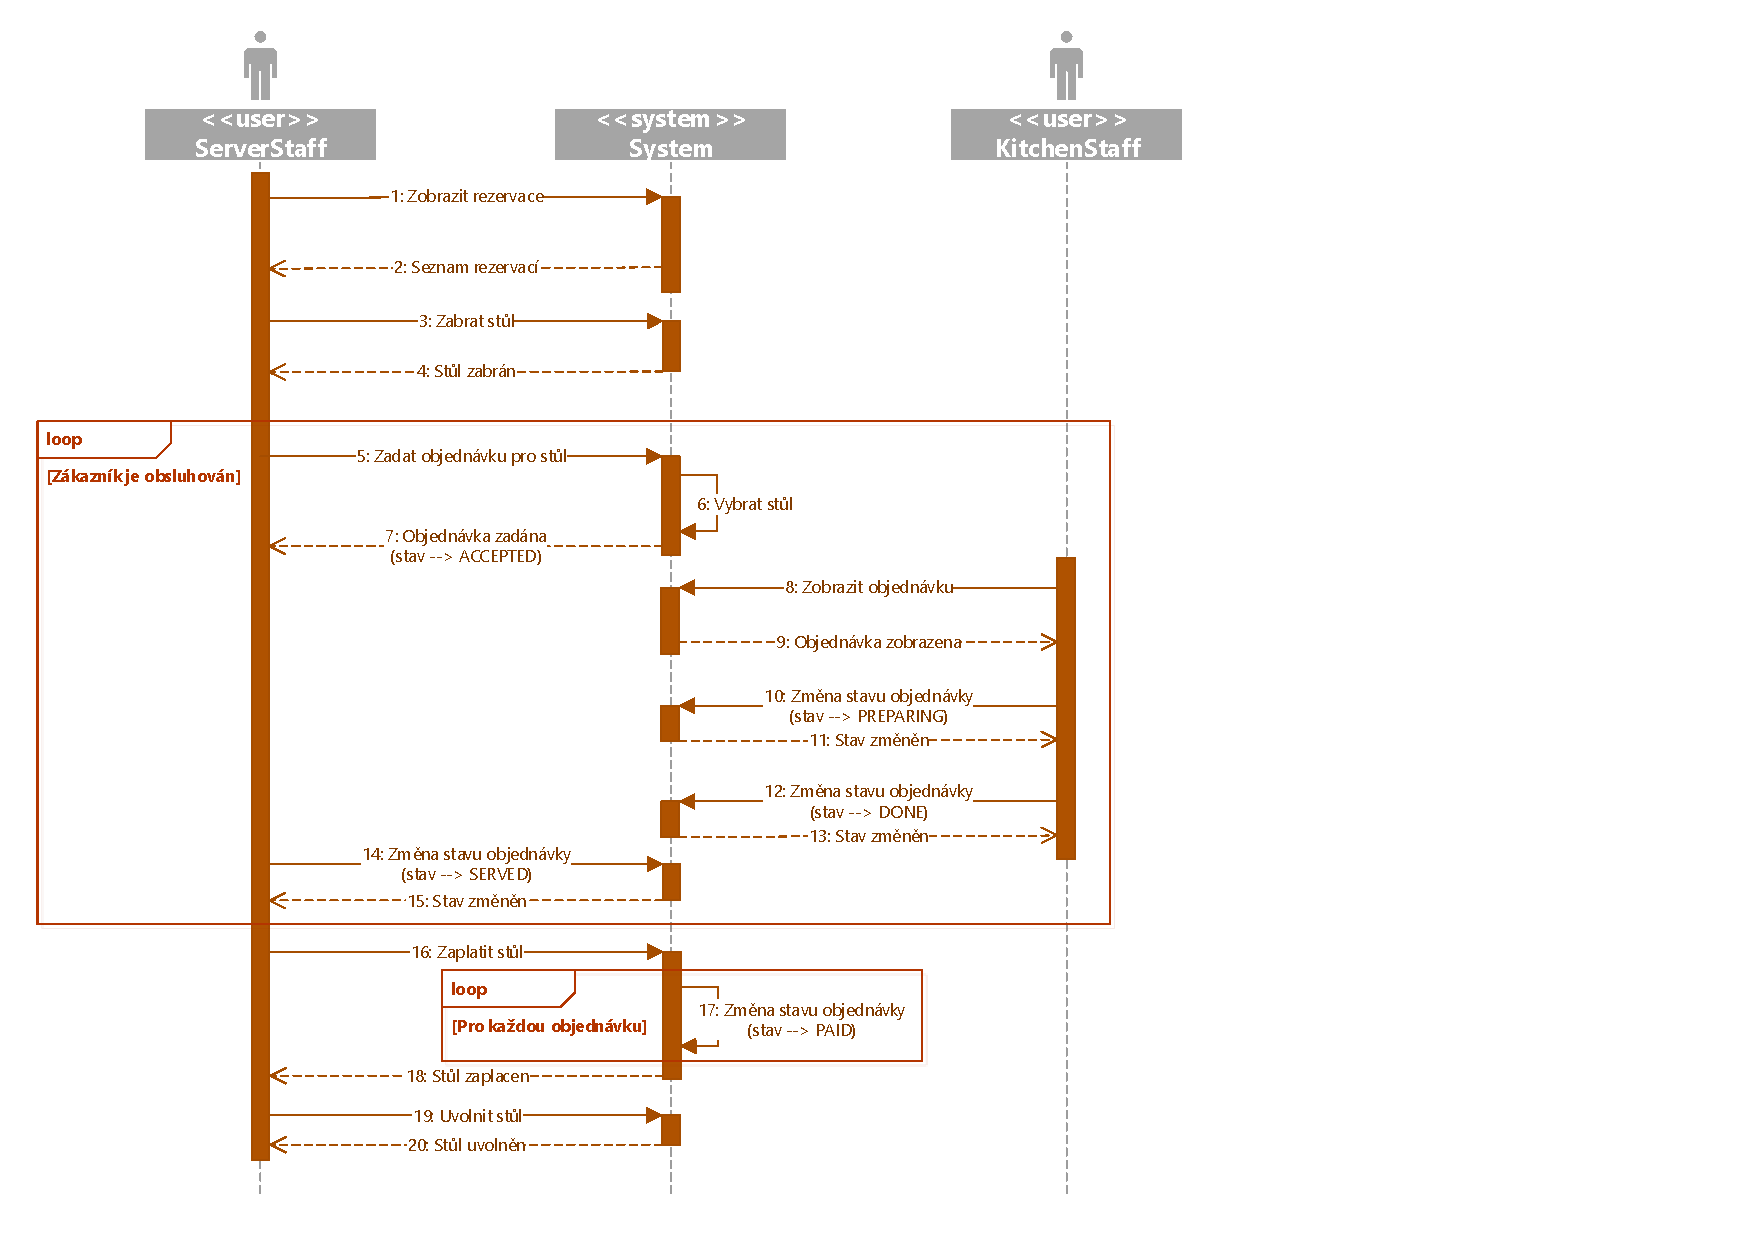
\includegraphics[scale=0.75]{../02_Vysledne_modely/04_SystemSequence.pdf}
\caption{Systémový diagram sekvence konkrétního scénáře: Obsluha zákazníka u stolu}
\label{fig:communication09-1}
\end{center}
\end{figure}


%%%%%%%%%%%%%%%%%%%%%%%%%%%%%%%%%%%%%%%%%%%%%%%%%%%%%%
%                05 DOMAIN CLASS DIAGRAM             %
%%%%%%%%%%%%%%%%%%%%%%%%%%%%%%%%%%%%%%%%%%%%%%%%%%%%%%
% TODO: Add path to the last iteration domain diagram
\newpage
\begin{figure}[h!]
\begin{center}
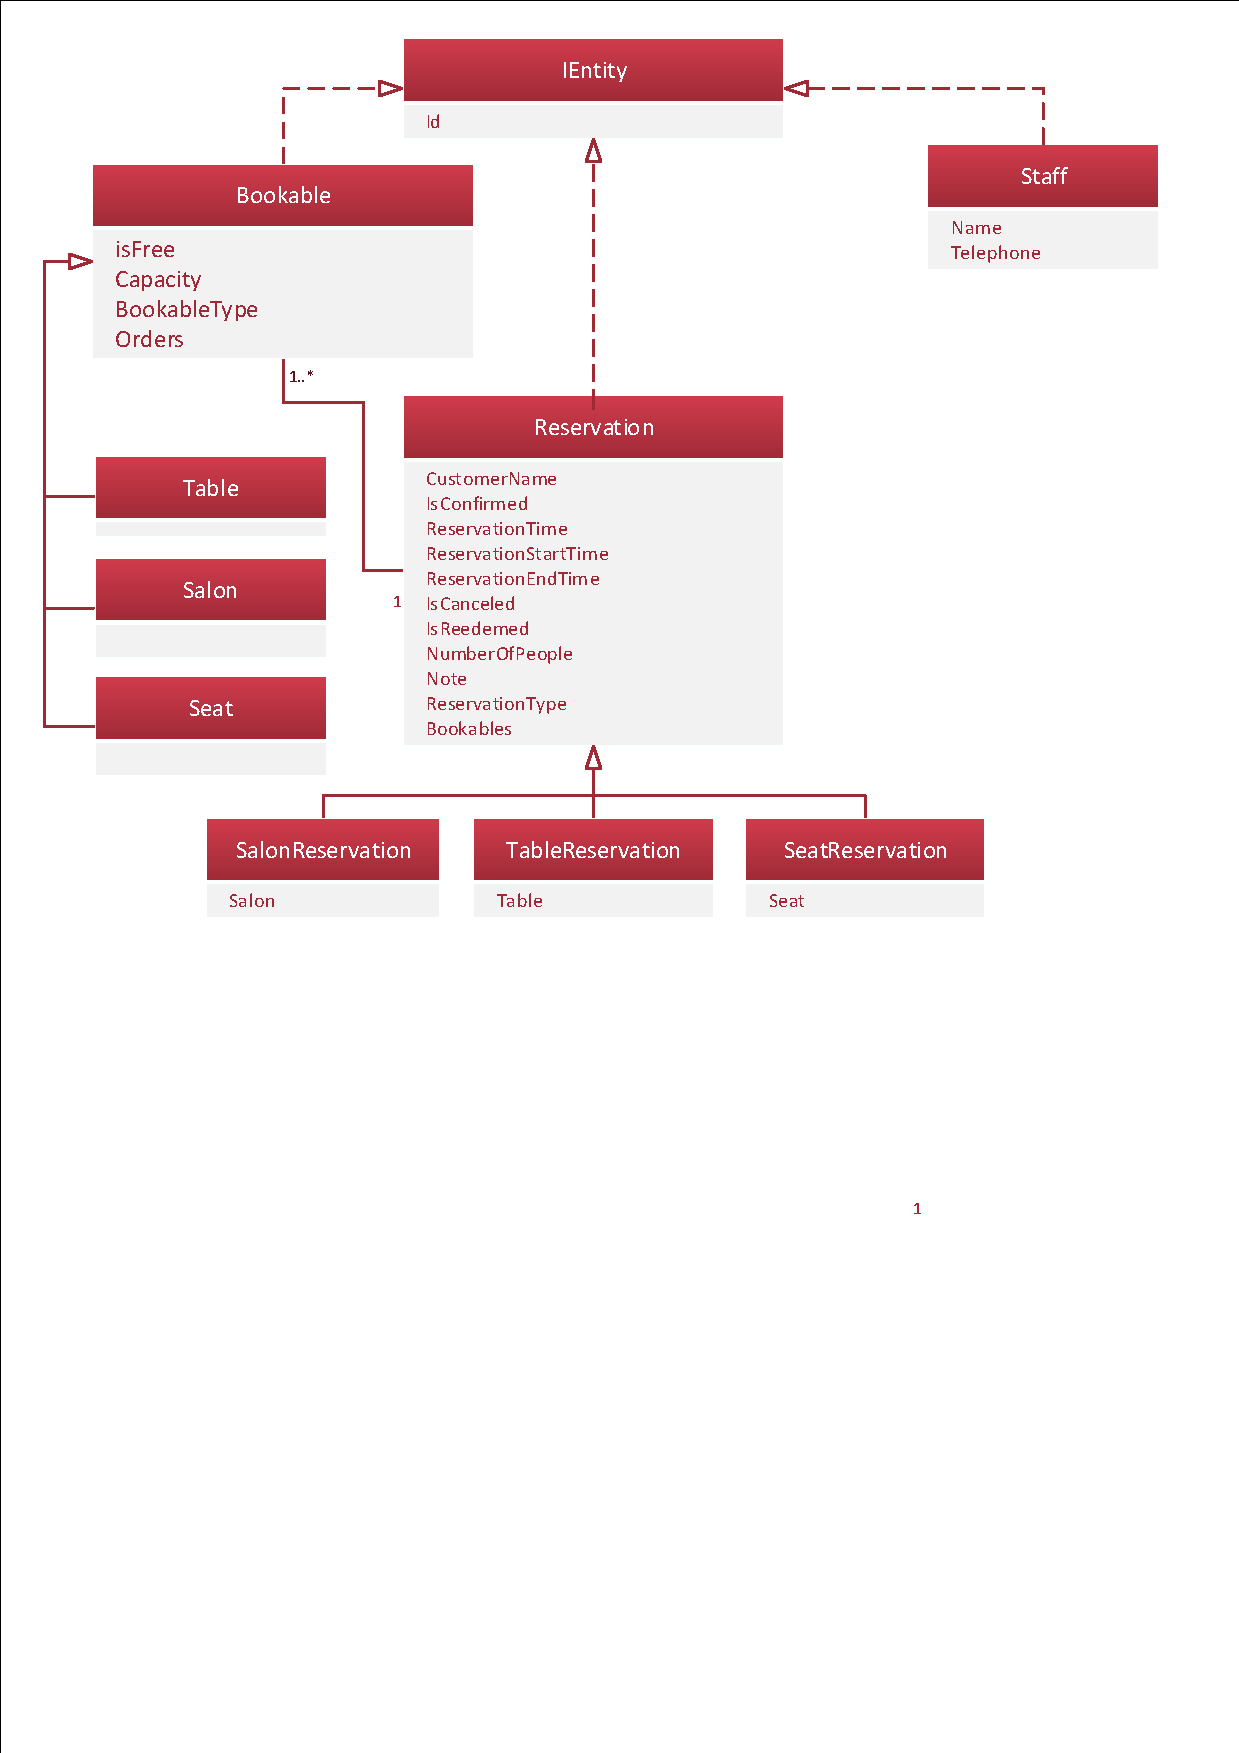
\includegraphics[scale=0.75]{../02_Vysledne_modely/05_1_ConceptualClassDiagram.pdf}
\vspace{-250pt}
\caption{Doménový konceptuální diagram tříd}
\label{fig:communication09-1}
\end{center}
\end{figure}


%%%%%%%%%%%%%%%%%%%%%%%%%%%%%%%%%%%%%%%%%%%%%%%%%%%%%%
%                06 TABLE OF RESPONSIBILITY          %
%%%%%%%%%%%%%%%%%%%%%%%%%%%%%%%%%%%%%%%%%%%%%%%%%%%%%%



%%%%%%%%%%%%%%%%%%%%%%%%%%%%%%%%%%%%%%%%%%%%%%%%%%%%%%
%                07 & 08 CLASS DIAGRAM               %
%%%%%%%%%%%%%%%%%%%%%%%%%%%%%%%%%%%%%%%%%%%%%%%%%%%%%%
\newpage
\begin{landscape}   
    \afterpage{
            
            \pagenumbering{gobble}

            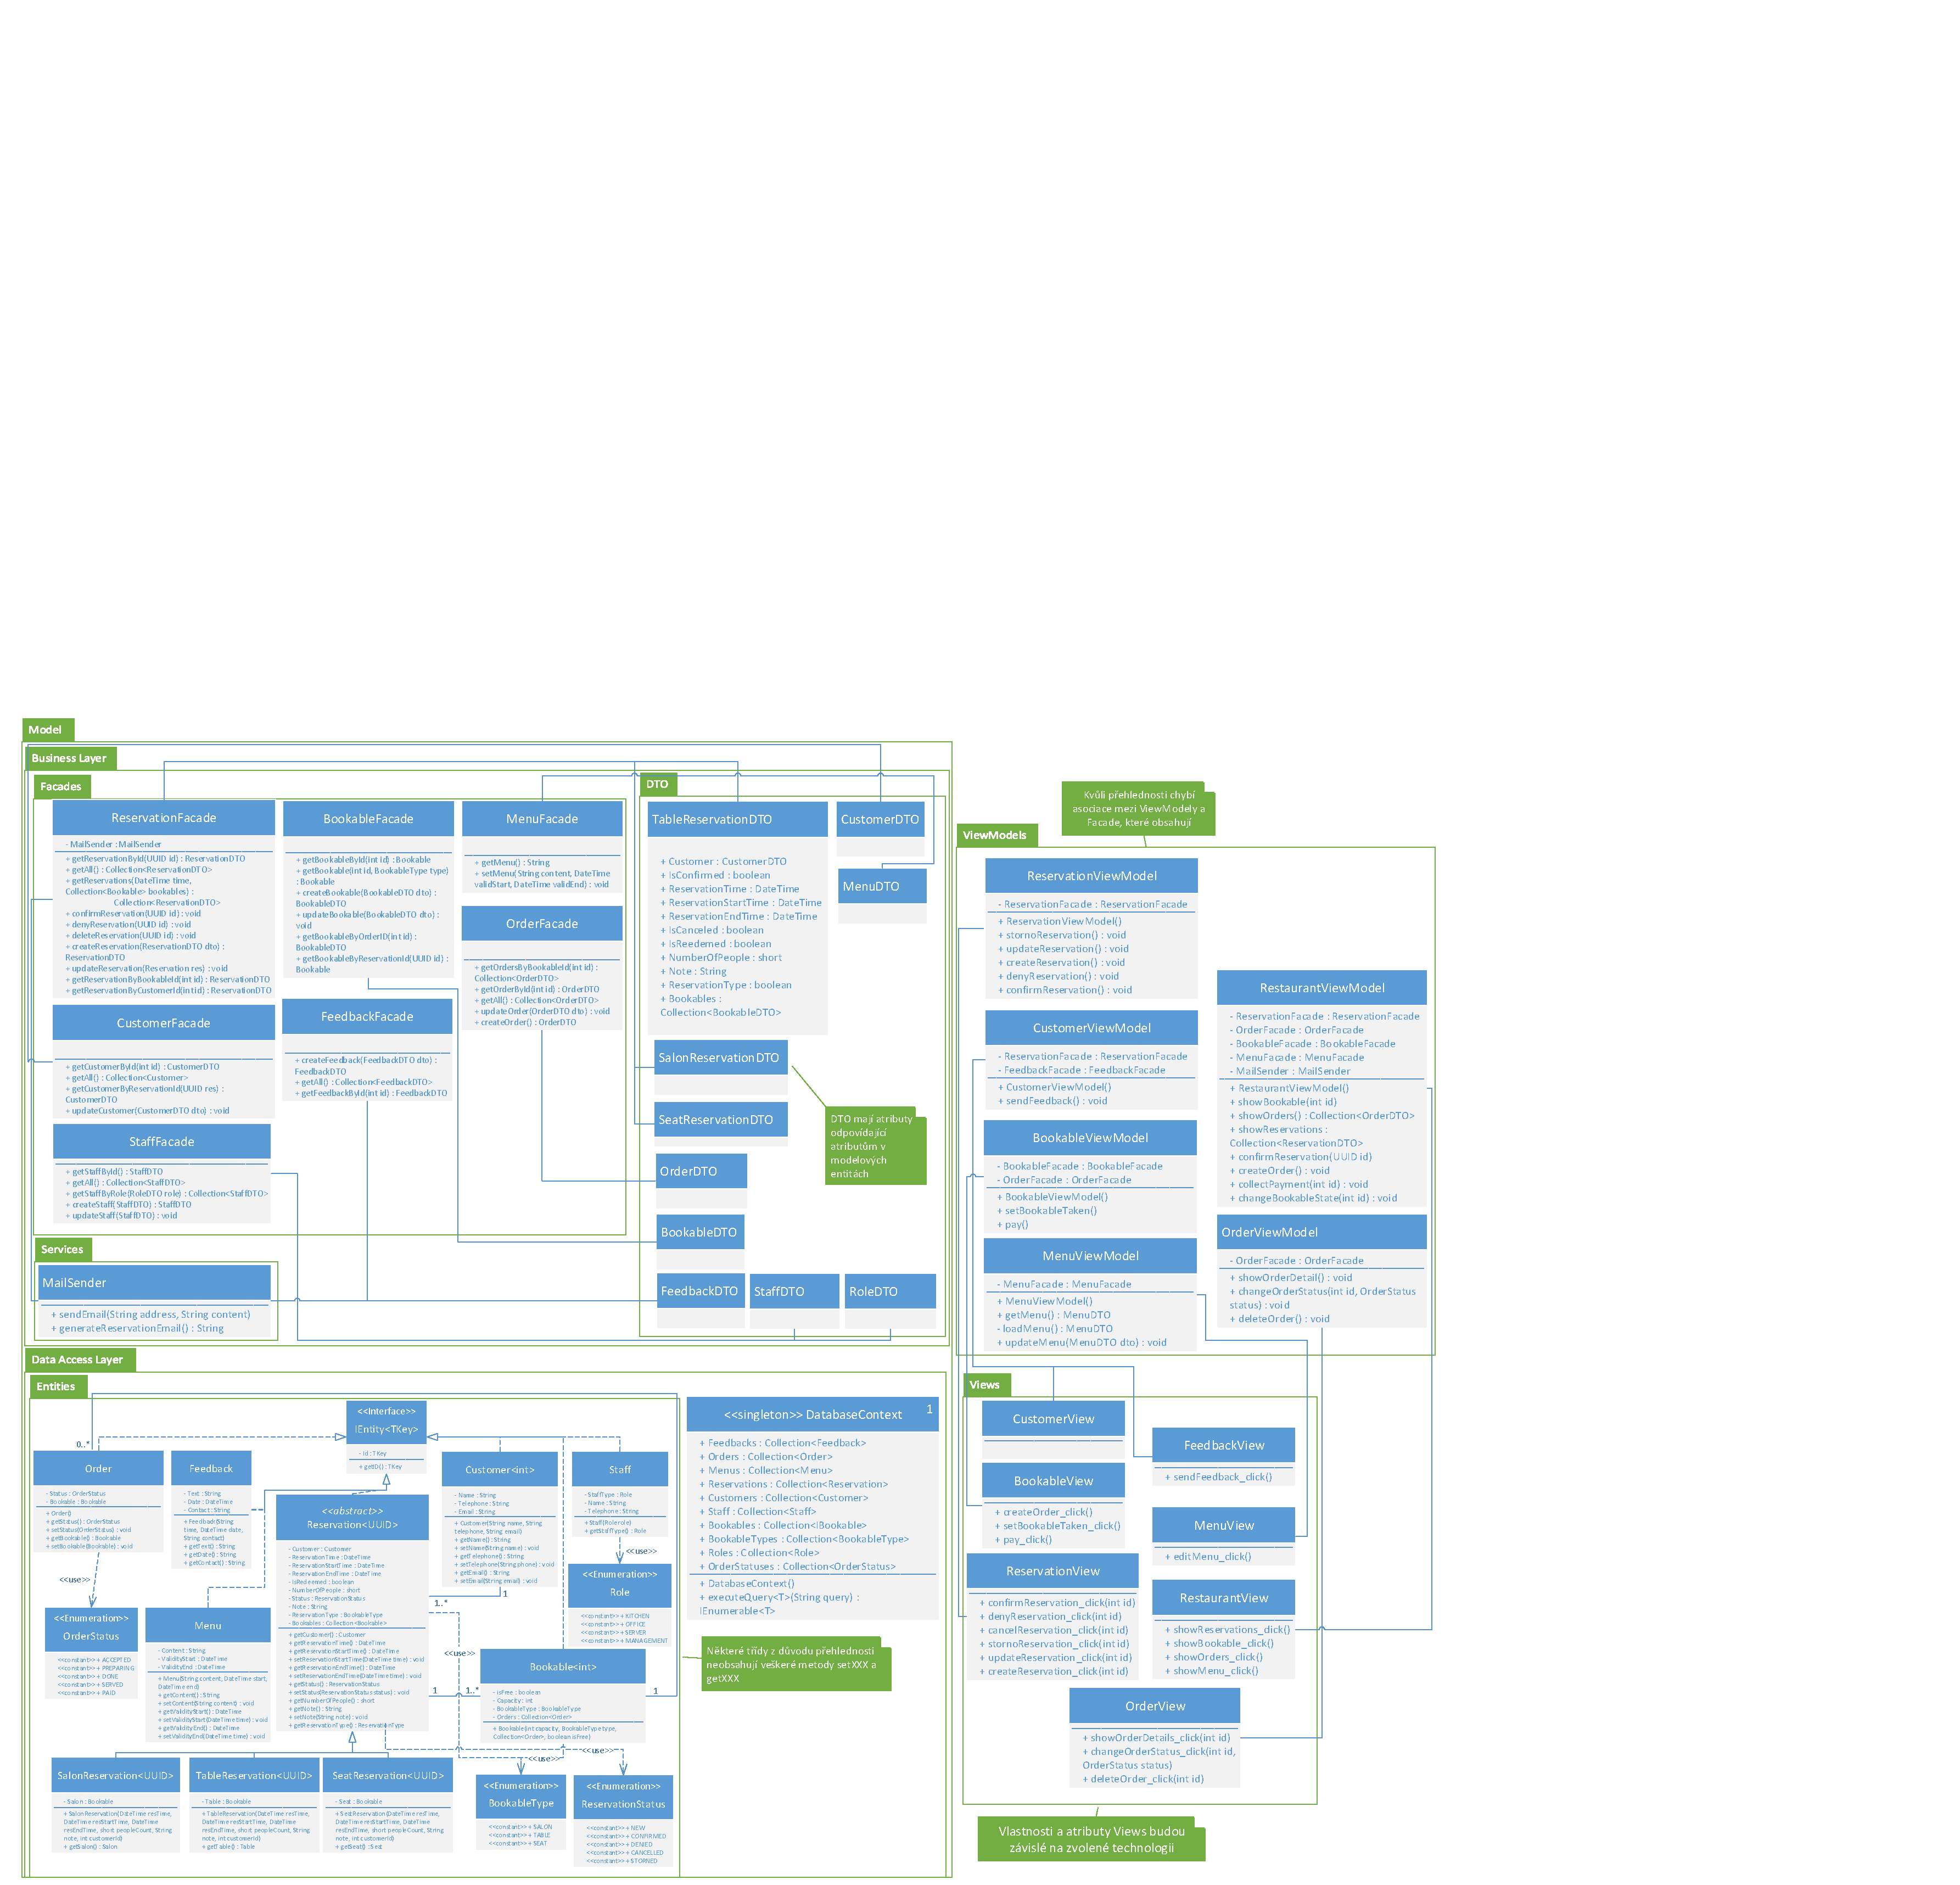
\includepdf[angle=90,scale=1]{../02_Vysledne_modely/07_ClassDiagram.pdf}
            \label{fig:iteration03}
        
            \clearpage
            \restoregeometry
        }
\end{landscape}



%%%%%%%%%%%%%%%%%%%%%%%%%%%%%%%%%%%%%%%%%%%%%%%%%%%%%%
%        09 DIAGRAMS 						         %
%%%%%%%%%%%%%%%%%%%%%%%%%%%%%%%%%%%%%%%%%%%%%%%%%%%%%%
\newpage
\begin{landscape}	
	\afterpage{
			
			\pagenumbering{gobble}

			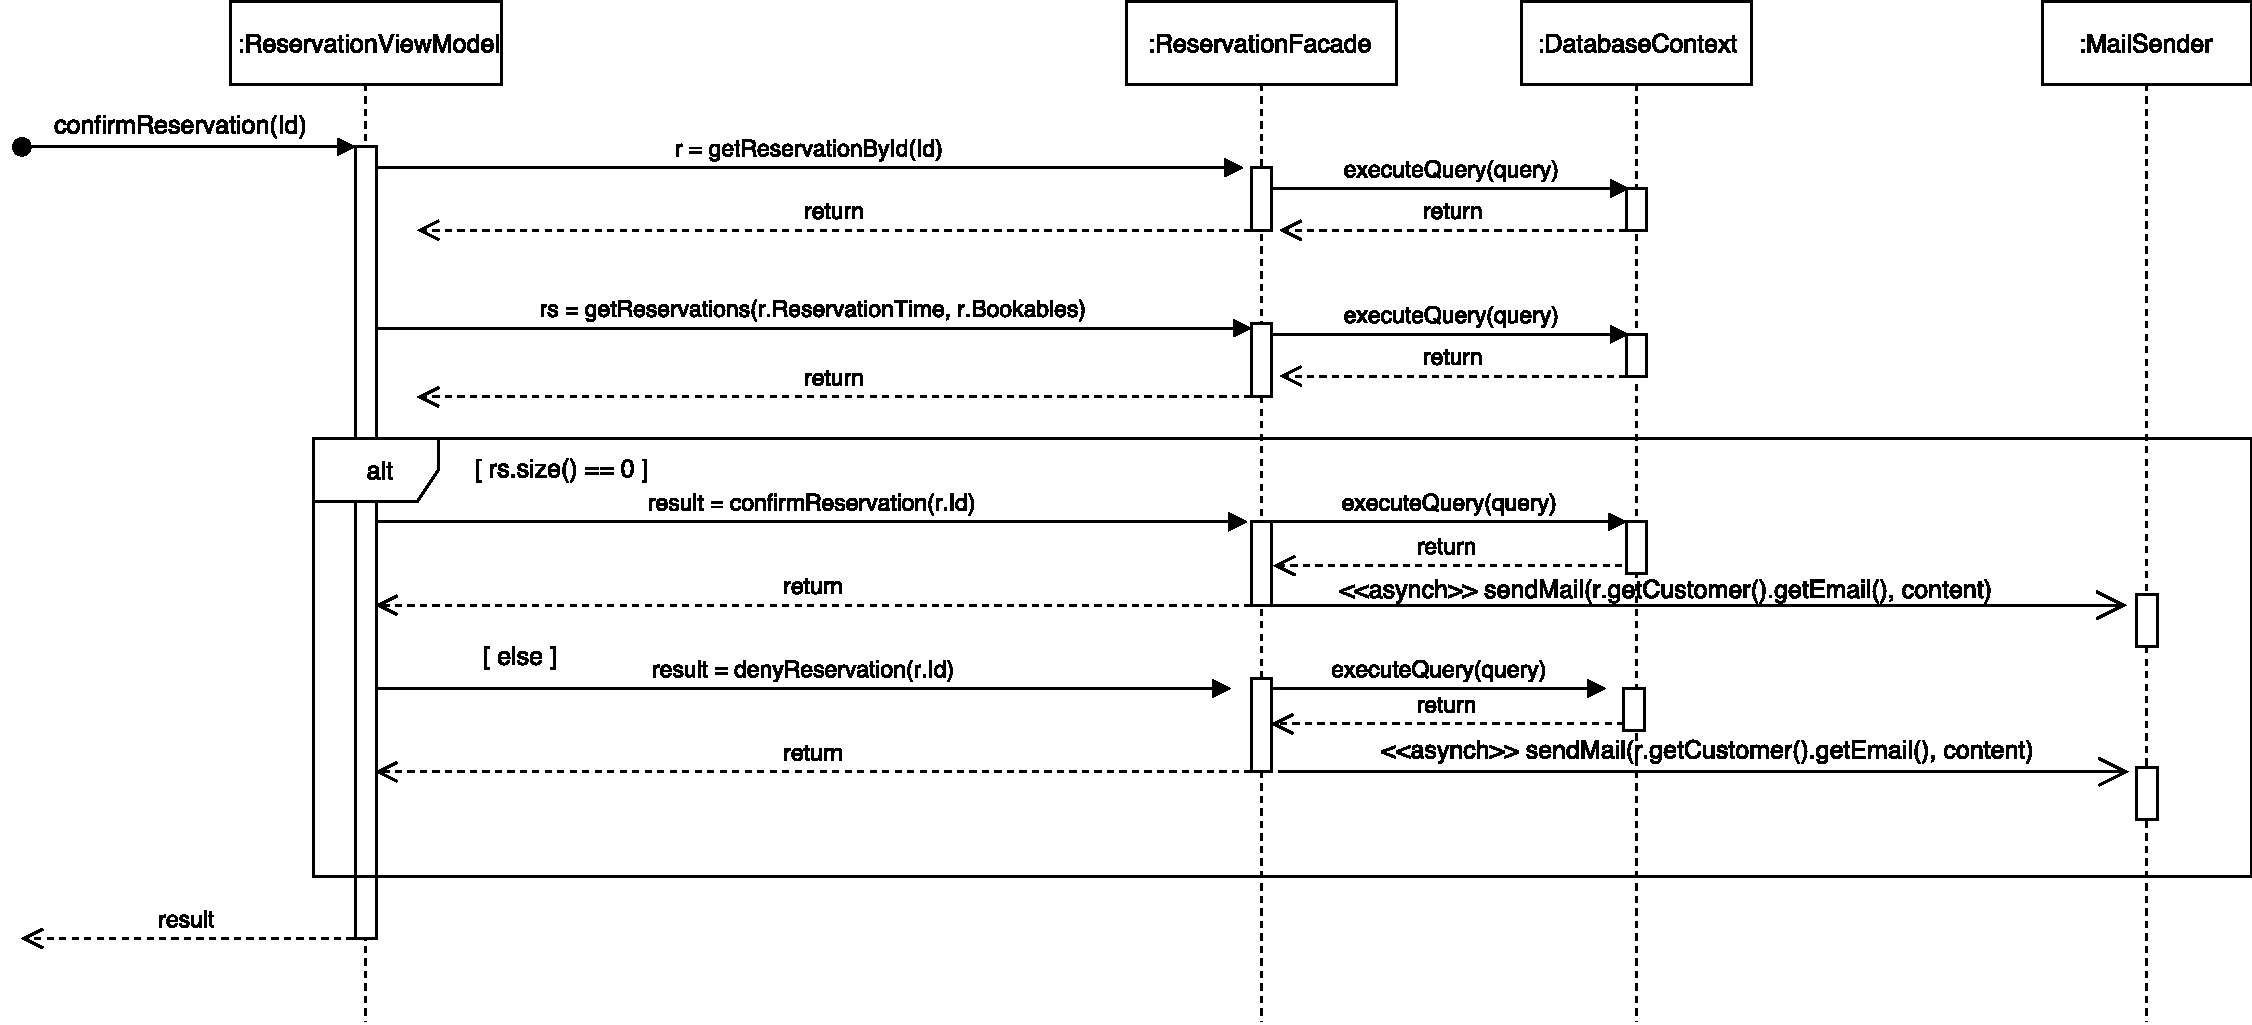
\includepdf[angle=90,scale=0.75,
				pagecommand={
					\thispagestyle{plain}
					\null\vfill
					\captionof{figure}{Diagram Sekvence pro potvrzení rezervace }}]{../02_Vysledne_modely/09_SequenceDiagram.pdf}
			\label{fig:iteration03}
		
			\clearpage
			\restoregeometry
		}
\end{landscape}

\newpage
\begin{landscape}	
	\afterpage{
			
			\pagenumbering{gobble}

			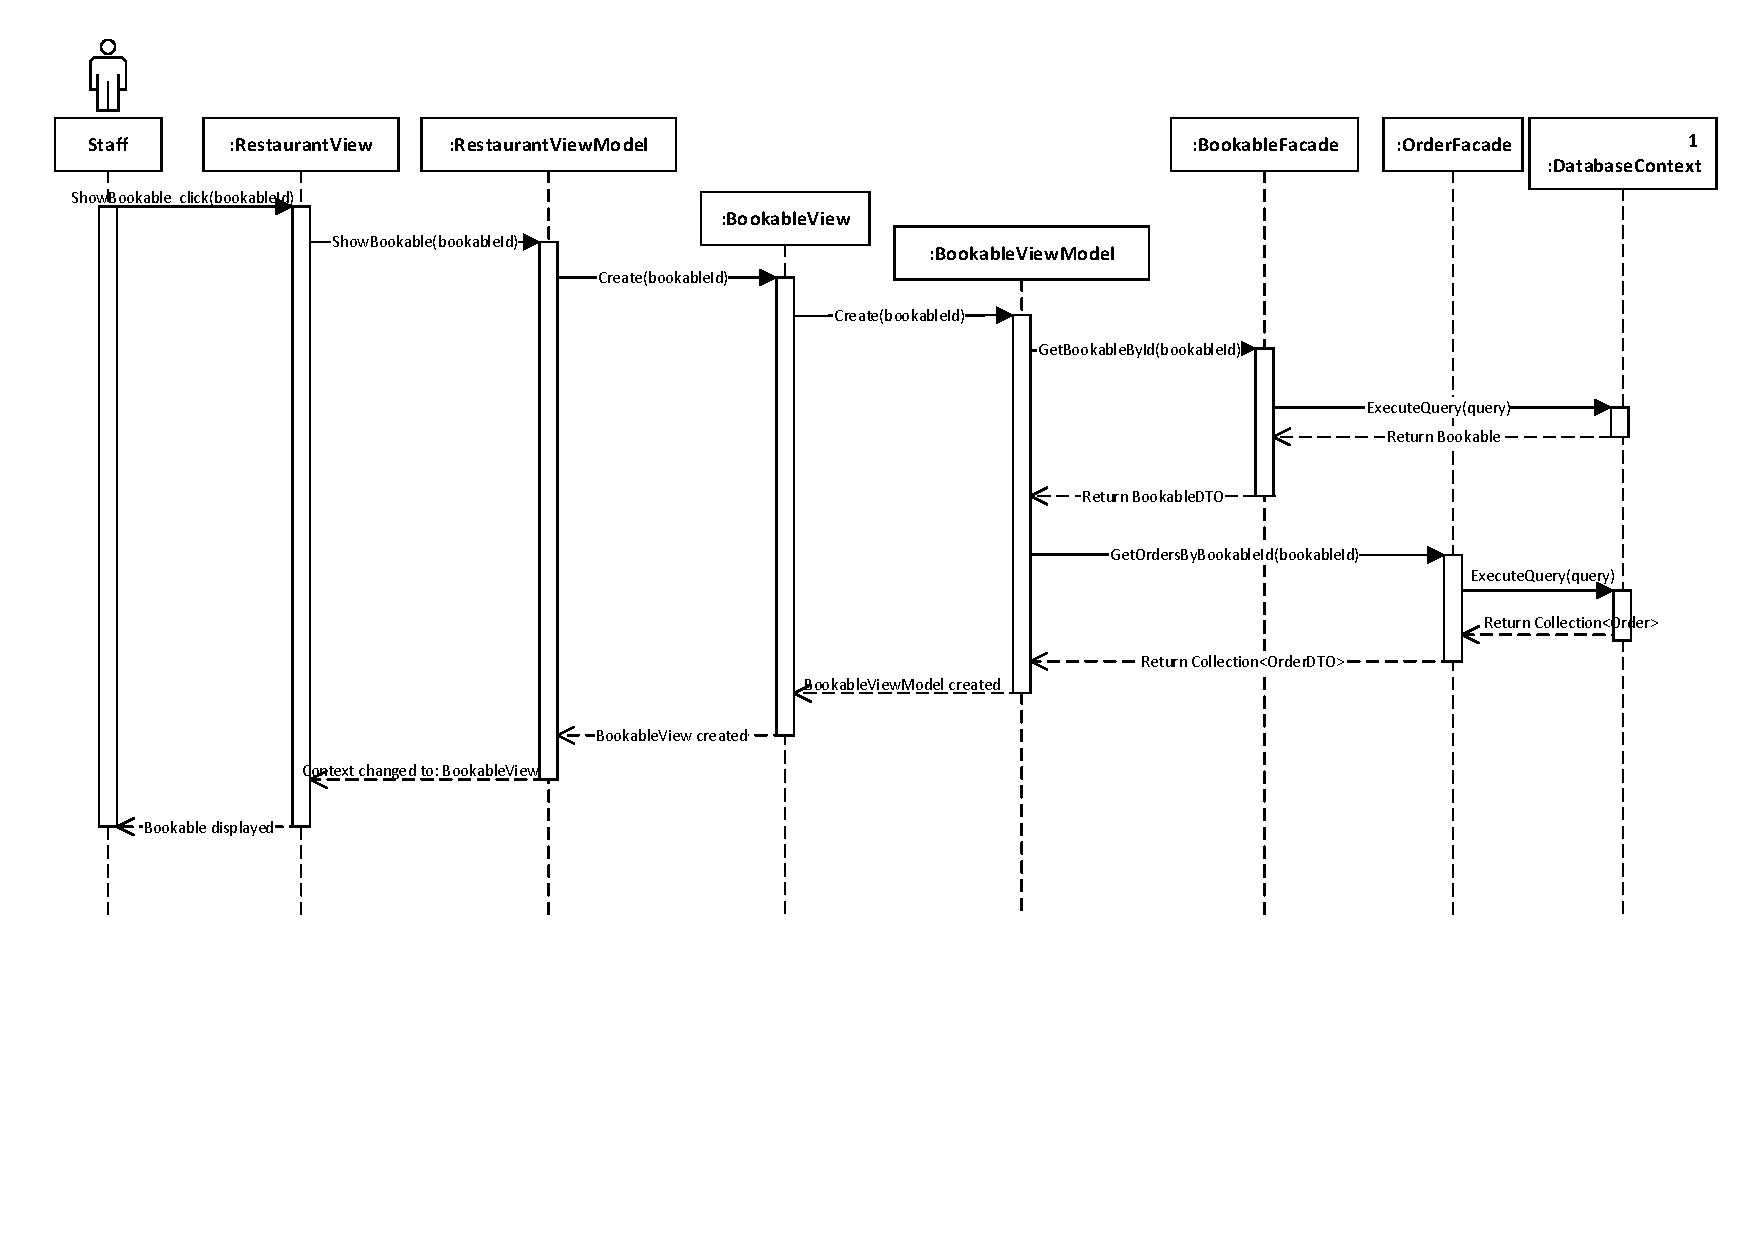
\includepdf[angle=90,scale=0.75,
				pagecommand={
					\thispagestyle{plain}
					\null\vfill
					\captionof{figure}{Diagram Sekvence pro potvrzení rezervace }}]{../02_Vysledne_modely/09_InteractionDiagram_SequenceDiagram_ShowBookable.pdf}
			\label{fig:iteration03}
		
			\clearpage
			\restoregeometry
		}
\end{landscape}

\newpage
\begin{figure}[h!]
\begin{center}
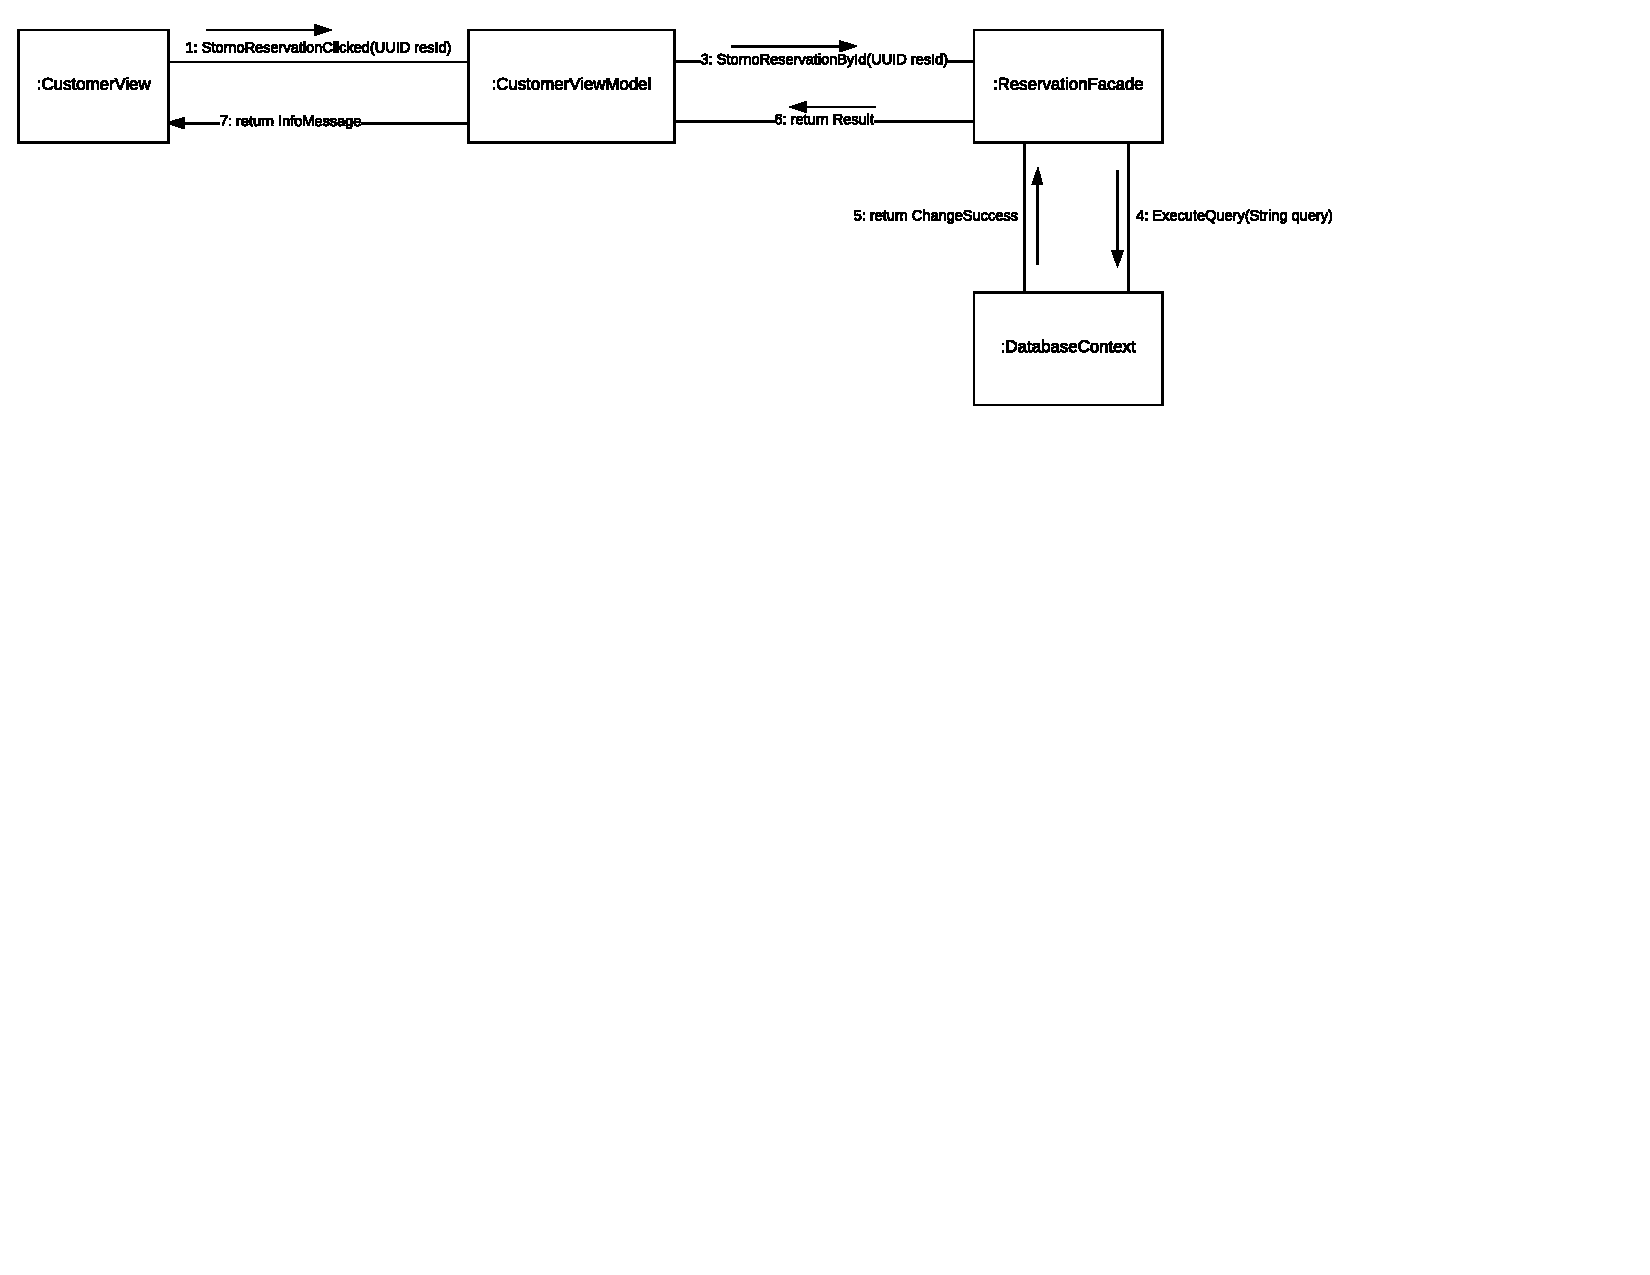
\includegraphics[scale=0.75]{../02_Vysledne_modely/09_CommunicationDiagram-1.pdf}
\vspace{-250pt}
\caption{Diagram Komunikace pro potvrzení rezervace}
\label{fig:communication09-1}
\end{center}
\end{figure}


%%%%%%%%%%%%%%%%%%%%%%%%%%%%%%%%%%%%%%%%%%%%%%%%%%%%%%
%        10 DIAGRAM NAVAZNOSTI OBRAZOVEK	 		 %
%%%%%%%%%%%%%%%%%%%%%%%%%%%%%%%%%%%%%%%%%%%%%%%%%%%%%%
\newpage
\begin{landscape}	
	\afterpage{
			
			\pagenumbering{gobble}

			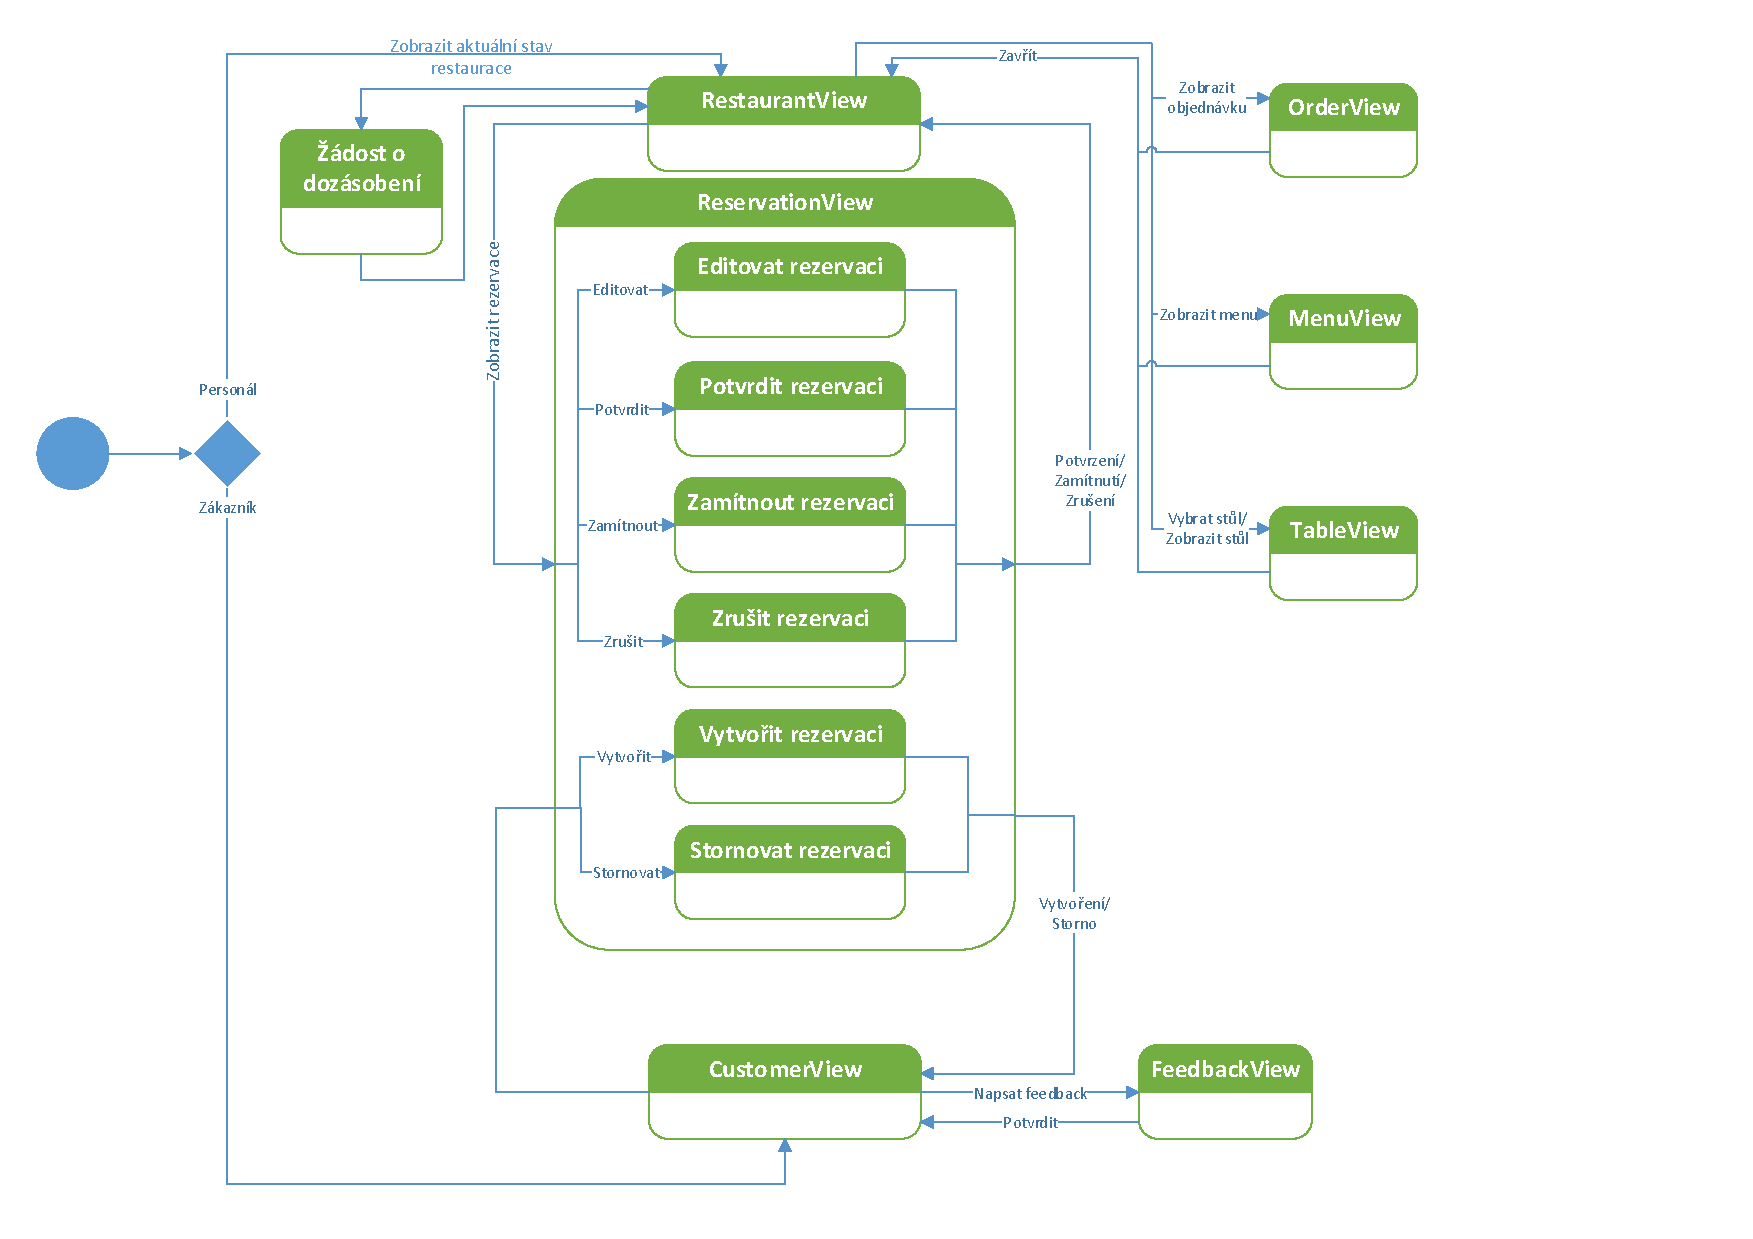
\includepdf[angle=90,scale=0.75,
				pagecommand={
					\thispagestyle{plain}
					\null\vfill
					\captionof{figure}{Model návaznosti jednotlivých obrazovek}}]{../02_Vysledne_modely/10_StateDiagram.pdf}
			\label{fig:iteration03}
		
			\clearpage
			\restoregeometry
		}
\end{landscape}
\newpage

%%%%%%%%%%%%%%%%%%%%%%%%%%%%%%%%%%%%%%%%%%%%%%%%%%%%%%
% 				11 Přejímací test 					 %
%%%%%%%%%%%%%%%%%%%%%%%%%%%%%%%%%%%%%%%%%%%%%%%%%%%%%%
\newpage
\section*{Přejímací testy}

% Přejímací test #1
{\large\textbf{Přejímací test 1: Zadat objednávku}} \\

\textbf{Popis}: \\\indent Uživatel systému (v roli Obslužný personál, nebo Vedení) zadává objednávku přijatou u stolu v restauraci. \\

\textbf{Předpoklady}: 
\begin{enumerate}
	\item Reálný Zákazník provedl objednávku v restauraci
	\item Obslužný personál nebo Vedení přijímá Zákazníkovu objednávku
\end{enumerate}

\textbf{Stav systému před provedením testu:}
\begin{enumerate}
	\item Systém běží a je responzivní.
	\item Databáze neobsahuje záznam o objednávce, kterou Obslužný personál nebo Vedení právě přijímá. 
\end{enumerate}

\textbf{Stav systému po provedení testu}:
\begin{enumerate}
	\item Systém běží a je responzivní.
	\item V databázi je vytvořen záznam o přijaté objednávce.
	\item V seznamu probíhajících objednávek se zobrazuje nově přijatá objednávka.
\end{enumerate}

\textbf{Postup}:
\begin{enumerate}
	% Krok #1
	\item 
	\begin{enumerate}
		\item Krok: Uživatel v roli Obslužný personál nebo Vedení otevře tlačítkem \uv{Zadat objednávku}
		\item Možné výstupy:
		\begin{enumerate}
			\item Úspěch: Systém zobrazí uživatelské rozhraní pro zadání nové objednávky.
			\item Neúspěch: Operace selže. 
			\item Neúspěch: Systém selže. 
		\end{enumerate} 
	\end{enumerate}

	% Krok #2
	\item 
	\begin{enumerate}
		\item Krok: Uživatel v roli Obslužný personál nebo Vedení vyplní informace o objednávce, včetně výběru stolu na otevřené obrazovce a klepne na tlačítko \uv{Zadat objednávku} pro potvrzení operace.
		\item Možné výstupy:
		\begin{enumerate}
			\item Úspěch: Systém vytvoří objednávku a zobrazí informační hlášku uživateli o úspěšném zadání objednávky.
			\item Neúspěch: Operace selže.
			\item Neúspěch: Systém selže.
		\end{enumerate} 
	\end{enumerate}

	% Krok #3
	\item 
	\begin{enumerate}
		\item Krok: Uživatel v roli Obslužný personál nebo Vedení vyplní informace o objednávce, bez výběru stolu na otevřené obrazovce a klepne na tlačítko \uv{Zadat objednávku} pro potvrzení operace.
		\item Možné výstupy:
		\begin{enumerate}
			\item Úspěch: Systém nevytvoří objednávku a zobrazí chybovou hlášku informující uživatele o chybějícím vyplněném stolu.
			\item Neúspěch: Systém vytvoří objednávku.
			\item Neúspěch: Operace selže.
			\item Neúspěch: Systém selže.
		\end{enumerate} 
	\end{enumerate}

	% Krok #4
	\item 
	\begin{enumerate}
		\item Krok: Uživatel v roli Obslužný personál nebo Vedení opraví dle instrukcí z předchozího kroku informace vyplněné na obrazovce zadávání objednávky a odešle objednávku tlačítkem \uv{Zadat objednávku}.
		\item Možné výstupy:
		\begin{enumerate}
			\item Úspěch: Systém vytvoří objednávku a zobrazí informační hlášku uživateli o úspěšném zadání objednávky.
			\item Neúspěch: Operace selže.
			\item Neúspěch: Systém selže.
		\end{enumerate} 
	\end{enumerate}
\end{enumerate}

% TODO: Make sure title and enumeration are on the same page 
\newpage
\textbf{Očekávaný výstup testu:} \\
\begin{enumerate}
	\item Krok 1 skončí výstupem (i) - Systém zobrazí uživatelské rozhraní pro zadání nové objednávky.
	\item Krok 2 skončí výstupem (i) - Systém vytvoří objednávku a zobrazí informační hlášku uživateli o úspěšném zadání objednávky.
	\item Krok 3 skončí výstupem (i) - Systém nevytvoří objednávku a zobrazí chybovou hlášku informující uživatele o chybějícím vyplněném stolu.
	\item Krok 4 skončí výstupem (i) - Systém vytvoří objednávku a zobrazí informační hlášku uživateli o úspěšném zadání objednávky.
\end{enumerate}


% Přejímací test #2
{\large\textbf{Přejímací test 2: Vytvořit rezervaci}} \\
\textbf{Popis}: \\\indent Zákazník rezervuje místo, popřípadě salón v restaurace na zvolené datum a čas. \\

\textbf{Předpoklady}: 
\begin{enumerate}
	\item Zákazník chce vytvořit rezervacii na místo, popřípadě salón v restauraci.
	\item Databáze rezervací je na začátku prázdná.
	\item Test probíhá v izolovaném prostředí, takže nepřichází konkurentní požadavky v průběhu tohoto testu.
\end{enumerate}

\textbf{Stav systému před provedením testu:}
\begin{enumerate}
	\item Systém běží a je responzivní.
	\item Systém dokáže zobrazit plánek restaurace s obsazenými místy.
	\item V databázi není informace o rezervaci Zákazníka. 
\end{enumerate}

\textbf{Stav systému po provedení testu}:
\begin{enumerate}
	\item Systém běží a je responzivní.
	\item V databázi je vytvořen záznam o žádosti o rezervaci.
	\item V seznamu objednávek čekajících na schválení je vidět Zákazníkem vytvořená rezervace.
\end{enumerate}

\textbf{Postup}:
\begin{enumerate}
	% Krok #1
	\item 
	\begin{enumerate}
		\item Krok: Zákazník klikne na odkaz \uv{Vytvořit rezervaci} 
		\item Možné výstupy:
		\begin{enumerate}
			\item Úspěch: Systém zobrazí uživatelské rozhraní pro vytvoření nové rezervace.
			\item Neúspěch: Operace selže. 
			\item Neúspěch: Systém selže. 
		\end{enumerate} 
	\end{enumerate}

	% Krok #2
	\item 
	\begin{enumerate}
		\item Krok: Zákazník vyplní informace o své osobě a čase kdy má zájem o rezervaci. 
		\item Možné výstupy:
		\begin{enumerate}
			\item Úspěch: Systém po ověření, že informace o čase je validní nabídne zobrazení plánku restaurace s dostupnými místy v daném čase.
			\item Neúspěch: Operace selže.
			\item Neúspěch: Systém selže.
		\end{enumerate} 
	\end{enumerate}

	% Krok #3
	\item 
	\begin{enumerate}
		\item Krok: Zákazník vybere volné místo v restauraci z plánku restaurace a odešle žádost o rezervaci kliknutím na tlačítko \uv{Rezervovat}
		\item Možné výstupy:
		\begin{enumerate}
			\item Úspěch: Systém vytvoří rezervaci.
			\item Neúspěch: Operace selže.
			\item Neúspěch: Systém selže.
		\end{enumerate} 
	\end{enumerate}

	% Krok #4
	\item 
	\begin{enumerate}
		\item Krok: Zákazník opět naviguje na formulář s vytvářením rezervace, vyplní jiné informace o své osobě, ale vybere stejný čas ve kterém má zájem o rezervaci.
		\item Možné výstupy:
		\begin{enumerate}
			\item Úspěch: Systém po ověření, že informace o čase je validní nabídne zobrazení plánku restaurace s dostupnými místy v daném čase. Místo, které Zákazník vybral v Kroku 2 je označené jako zabrané.
			\item Neúspěch: Systém po ověření, že informace o čase je validní nabídne zobrazení plánku restaurace s dostupnými místy v daném čase. Místo, které Zákazník vybral v Kroku 2 je označené jako nezabrané.
			\item Neúspěch: Operace selže.
			\item Neúspěch: Systém selže.
		\end{enumerate} 
	\end{enumerate}

	% Krok #5
	\item 
	\begin{enumerate}
		\item Krok: Zákazník nevybere žádné místo a odešle rezervační formulář tlačíkem \uv{Rezervovat}.
		\item Možné výstupy:
		\begin{enumerate}
			\item Úspěch: Systém zobrazí chybovou hlášku informující uživatele o nutnosti vybrat místo z plánku restaurace.
			\item Neúspěch: Systém odešle rezervaci na nula míst.
			\item Neúspěch: Operace selže.
			\item Neúspěch: Systém selže.
		\end{enumerate} 
	\end{enumerate}
\end{enumerate}

\textbf{Očekávaný výstup testu:} \\
\begin{enumerate}
	\item Krok 1 skončí výstupem (i) - Systém zobrazí uživatelské rozhraní pro vytvoření nové rezervace..
	\item Krok 2 skončí výstupem (i) - Systém po ověření, že informace o čase je validní nabídne zobrazení plánku restaurace s dostupnými místy v daném čase.
	\item Krok 3 skončí výstupem (i) - Systém vytvoří rezervaci.
	\item Krok 4 skončí výstupem (i) - Systém po ověření, že informace o čase je validní nabídne zobrazení plánku restaurace s dostupnými místy v daném čase. Místo, které Zákazník vybral v Kroku 2 je označené jako zabrané.
	\item Krok 5 skončí výstupem (i) - Systém zobrazí chybovou hlášku informující uživatele o nutnosti vybrat místo z plánku restaurace..
\end{enumerate}
